\chapter{SDN control mechanism evaluation}
\ifpdf
    \graphicspath{{Chapter1/Chapter1Figs/PNG/}{Chapter1/Chapter1Figs/PDF/}{Chapter1/Chapter1Figs/}}
\else
    \graphicspath{{Chapter1/Chapter1Figs/EPS/}{Chapter1/Chapter1Figs/}}
\fi

This chapter contains the results of an exhaustive characterisation study of
existing SDN technologies. We are trying to understand the capabilities of the
SDN paradigm as well as the limitation incurred by current implementation
efforts. The work focuses on the functionality of version 1.0 of the \of
protocol, as the sole protocol instatiation of this technology. 
% This is the sole standardised instantiation of the SDN paradigm and
% version 1.0 is the current standard available in hardware switches.  \of
% functionality is modular, thus the experiments can be reproducible over other
% future SDN protocol specifications.  
For this work, we have developed two
frameworks: \oflops and \sdnsim. \oflops is a high precision \of switch
micro-benchmark platform. Using the platform, we develop a set of elementary
testing scenario in order to understand the performance limitation of existing
\of switch implementations.  \sdnsim is a macro-benchmark platform for \of
architectures. The platform extends the Unikernel abstraction in order to
support large scale network simulation and emulation, using the same experiment
specification. 

In this Chapter, we firsty present the motivations (Section~\ref{sec:oflops-intro}) and
the design overview of the \oflops platform (Section~\ref{sec:oflops-design}).
Further, we select a number of off-the-self \of implementations
(Section~\ref{sec:oflops-switches}) and present the results of \oflops test
scenarios over the elemenetary interactions provided by the protocol
(Section~\ref{sec:oflops-result}). Furthermore, in order to study the results
extracted from the oflops platform in a macroscopic level, we present the
\sdnsim platform (Section~\ref{sec:sdnsim-intro}) and its design
(Section~\ref{sec:sdnsim-design}). Finally, we analyse the performance of the
\sdnsim implementation and employ it to evaluate network control approaches in a
fat-tree topology (Section~\ref{sec:sdnsim-precision}) and conclude
(Section~\ref{sec:conclusion}). 

%% We can see that the architecture of the Mirage switch
%% has no impact in the switching performance and is similar with the
%% performance of ovs. Furthermore, we note that when we use a 1 Mbps
%% packet probe we notice that both switches exhibit a high per packet
%% processing delay. We believe that this is due to the underlying
%% bridging functionality of the Dom0 network stack. We have to point out
%% though, that the mirage switch is able to run with minimum memory
%% requirements. Specifically, the switch is able to run and function
%% using only 32 Mbytes of memory, while the openvswitch vm requires at
%% least 128 Mbytes in order to boot up.We are currently working towards
%% developing a better integration of the switch functionality with the
%% network stack of xen in order to achieve lower switching latency.


% SDN context
% Driven by the OpenFlow
% initiative\footnote{\url{http://www.openflow.org/}}, the
% Software-Defined Networking (SDN) paradigm is gearing towards the
% definition of a standard way of providing pragrammatic control of
% network devices. Recently, the Open Networking Foundation
% \footnote{\url{http://www.opennetworkingfoundation.org/}} (ONF) was
% formed and is supported by major Internet companies including
% Microsoft, Google, Facebook, Cisco, Juniper, and VMware. With the
% ONF's first priority being to develop and use the OpenFlow protocol, a
% large number of commercial hardware platforms can be expected to
% become SDN-enabled in the near future.

% intro about SDN
\section{\oflops introduction} \label{sec:oflops-intro}

% OpenFlow\footnote{\url{http://www.openflow.org/}}, an instance of
% software-defined networking (SDN), gives access deep within the network
% forwarding plane while providing a common, simple, API for network-device
% control. Implementation details are left to the discretion of each vendor. This
% leads to an expectation of diverse strengths and weaknesses across the existing
% OpenFlow implementations, which motivates our work.


% As we have discussed in Chapter~\ref{ch:background}, SDN techology can
% enhance the functional capabilities of a network and provide high resolution 
% flow control mechanisms in order to fulfil network application requirements. 
% Although the short period since the introduction of the SDN paradigm, 
% many novel control architectures have been proposed~\cite{plug_n_serv,difane,flowvisor-osdi}. 
% One the most successful instantiations of the SDN paradigm is the \of protocol, 
% standardized and developed by a joint consortium of educational and industrial
% institutes, the Open Network Foundation (ONF). Currently \of is the sole SDN 
% protocol that provides production support from a wide range of network vendors, 
% while educational funding in US~\cite{ofelia} and Europe~\cite{ofelia} have 
% develops large scale \of testbeds in order to support earch nnovativation in the
% field.

%\of is increasingly adopted, both by hardware vendors as well as by the
%research community \cite{plug_n_serv,difane,flowvisor-osdi}.

Although the short period since the introduction of the SDN paradigm, many novel
control architectures have been
proposed~\cite{plug_n_serv,difane,flowvisor-osdi}. The deployment of such
architectures to production networks isn't straightforward. 
In~\cite{Weissmann:va} authors describe their experience
in deploying the first \of production networks in Stanford University and point
out that the initial deployment was highly under-performing and unreliable when
a simple reactive control scheme was deployed. The main source of problems
relates to firmware and hardware limitations. In order though to make the
transition of SDN and \of from research to industry ,  developers need to
evaluate thoroughly proposed functionality and provide accurate availability and
performance guarantees. In order to address this issue we developed
\oflops~\footnote{\oflops is under GPL licence and can be downloaded from
  \url{http://www.openflow.org/wk/index.php/Oflops}}, a measurement framework
that enables rapid development of use-case tests for both hardware and software
OpenFlow switch implementations. To better understand the behavior of the tested
OpenFlow implementations, \oflops combines measurements from the OpenFlow
control channel with data-plane measurements. To ensure sub-millisecond-level
accuracy of the measurements, we bundle the \oflops software with specialized
hardware in the form of the NetFPGA
platform\footnote{\url{http://www.netfpga.org}}.  Note that if the tests do not
require millisecond-level accuracy, commodity hardware can be used instead of
the NetFPGA \cite{pam-accuracy}.

% We use \oflops to test publicly available OpenFlow software
% implementations as well as several OpenFlow-enabled commercial hardware
% platforms, and report our findings about their varying performance
% characteristics.  

% I would remove the following paragraph, this is not very relevant.
%The SDN concept has been employed by several authors to introduce innovation 
% in the forwarding behavior of the network. For example, 
%Greenhalgh~\etal.~\cite{flowstream} build a flexible flow
%processing platform based on commodity hardware. Handigol~\etal~\cite{plug_n_serv} 
%demonstrate a Web traffic load-balancer based on OpenFlow. 
%Yu~\etal~\cite{difane} scale
%flow-switching in an enterprise network by distributing the flow rules
%across the different switches. Sherwood~\etal~\cite{flowvisor-osdi}
%augment OpenFlow with flow-space isolation.


% What we propose in this paper: exploit the SDN paradigm to measure SDN capabilities.
%\todo{reviewer: you either make the case that SDN has "more and more promising use-cases" 
%or you say that you want to "help SDN become relevant"}
%While more and more promising use-cases for SDN technology are being
%proposed, the capabilities and performance delivered by SDN-enabled
%hardware is largely unknown. The history of networking has repeatedly
%reminded the research community that it takes time between innovations
%are proposed and the corresponding real-world applications are being
%deployed, e.g., multicast, VoIP, IPv6. To help SDN become a relevant
%technology in the real-world, we propose a framework that allows
%SDN-based application developers to test the actual capabilities of
%SDN hardware.

% The rest of this paper is structured as follows. We first present the design
% of the \oflops framework in Section~\ref{sec:design}. We describe the 
% measurement setup in Section~\ref{sec:switches}. We describe our measurements
% in Section~\ref{sec:results}. We provide basic experiments that test the flow
% processing capabilities of the implementations (Section~\ref{sec:results-packets})
% as well as the performance and overhead of the OpenFlow communication channel 
% (Section~\ref{sec:results-rate}). We follow with specific tests, targeting the monitoring
% capabilities of OpenFlow (Section~\ref{sec:results-monitoring}) as well as interactions
% between different types of OpenFlow commands (Section~\ref{sec:results-interactions}).
% We conclude in Section~\ref{sec:conclusion}.
% Rest of this paper...

\section{\oflops design}\label{sec:oflops-design}

Measuring OpenFlow switch implementations is a challenging task in terms of
characterization accuracy, noise suppression and precision.  Performance
characterization is not trivial as most OpenFlow-enabled devices provide rich
functionality but do not disclose implementation details. In order to understand
the performance impact of an experiment, multiple input measurements must be
monitored concurrently. Further, current controller designs,
like~\cite{Gude08,SNAC}, target production networks and thus are optimized for
throughput maximization and programmability, but incur high measurement
inaccuracy. Measurement noise suppresion in the control plane requires 
a new simplified \of controller library with low processing
latency. Finally, high precision measurements after a point are subject to loss
due to unobserved parameters of the measurement host, such as OS scheduling and
clock drift. The result of these challenges is that meaningful, 
controlled, repeatable performance tests are non-trivial in an \of
environment.

% Since the beggining of our measurement study, it became apparent to us
% that the assesment of OpenFlow implementations is not trivial and it
% has a number of challenges.  Firstly, in order to assess the
% performance and understand the limitations of a network device that
% has both rich functionality and for which we have little idea of the
% implementation, multiple input measurement should be monitored
% concurently in order to encompass all parameters of an
% experiment. Secondly, OpenFlow controllers like \cite{Gude08,SNAC}
% provide advanced APIs that support fine-grained control of the switch,
% through extensions based upon language mechanisms such as C++ bindings
% to Python. As a result, such extensions introduce processing
% complexity on the control channel which may introduce measurement
% noise, making them inappropriate for our measurements. Finally, for
% some of our measurements we required fine time precision, which after
% a point is subject to losses due to measurement host parameters, such
% as OS scheduling.


\begin{figure}
\centering
\begin{minipage}[b]{0.49\linewidth}
\centering
 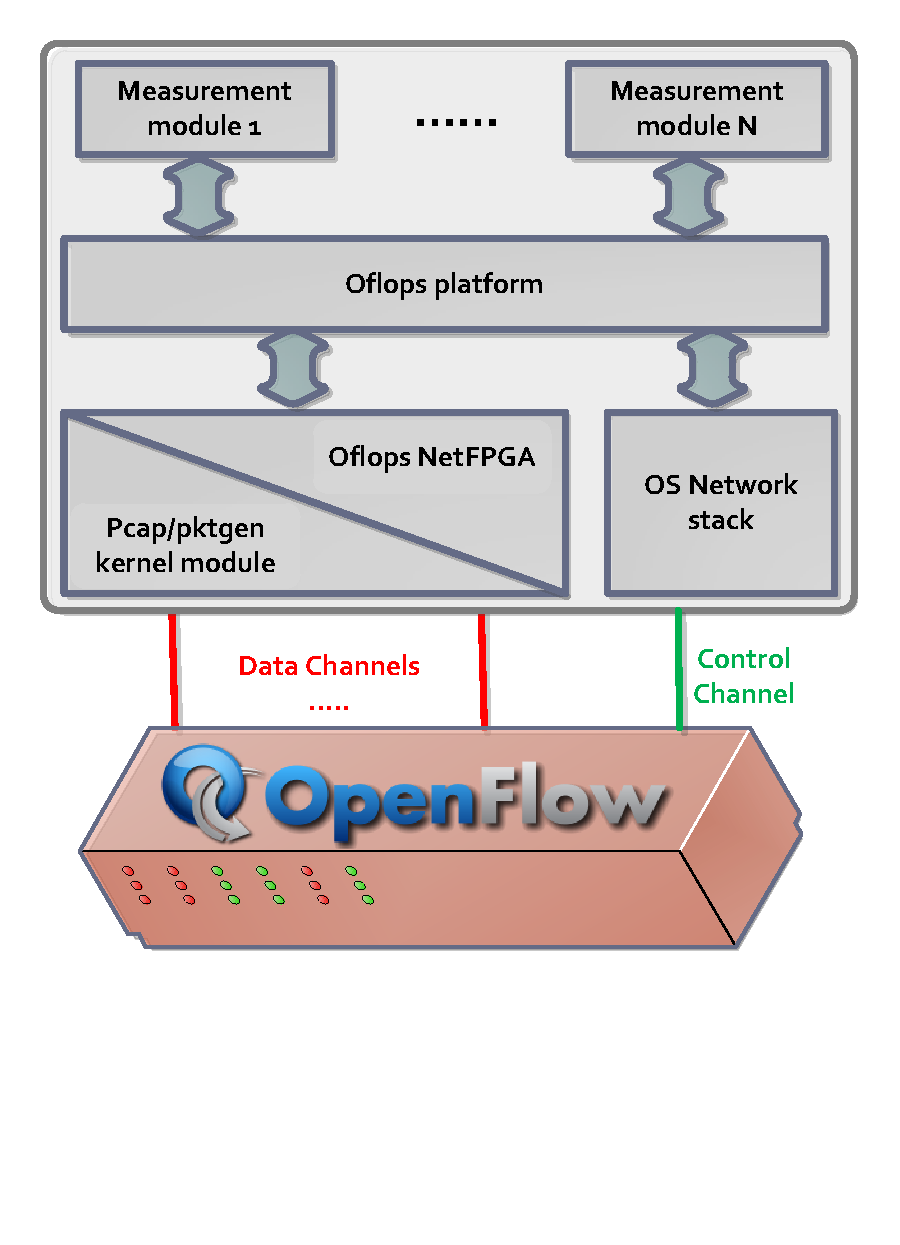
\includegraphics[width=0.99\textwidth]{openflow-design} 
\caption{\oflops design schematic}
\label{fig:oflops_design}
\end{minipage}
\begin{minipage}[b]{0.49\linewidth}
\centering
 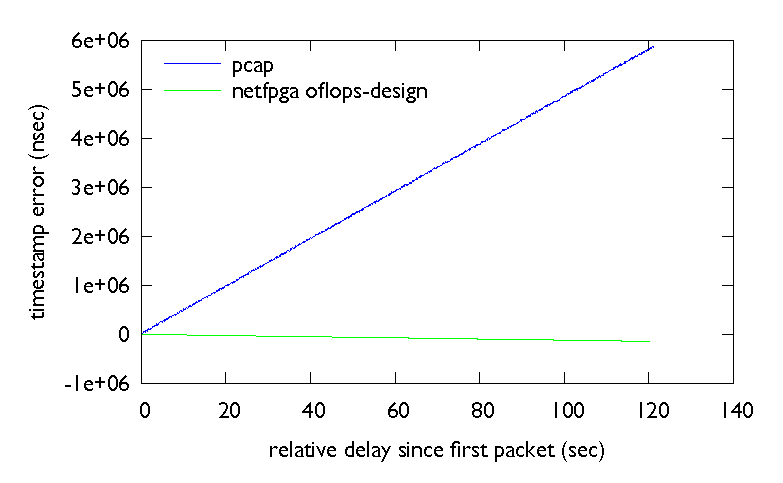
\includegraphics[width=0.99\textwidth]{timer_precision} 
 \caption{Evaluating timestamping precision using a DAG card.}
\label{fig:timestamping}
\end{minipage}
\end{figure}

The \oflops design philosophy aims to develop a low overhead abstraction layer
that allows interaction with an OpenFlow-enabled device over multiple data
channels.  The platform provides a unified system that allows developers to
control and receive information from multiple control sources: data and control
channels as well as SNMP to provide specific switch-state information.
For the development of measurement experiments over \oflops, the platform
provides a rich, event-driven, API that allows developers to handle events
programatically in order to implement and measure custom controller
functionality. The current version is written predominantly in C. Experiments
are compiled as shared libraries and loaded at run-time using a simple
configuration language, through which experimental parameters can be defined.
A schematic of the platform is presented in Figure~\ref{fig:oflops_design}.
Details of the \oflops programming model can be found in the API manual
\cite{oflops-manual}.

The platform is implemented as a multi-threaded application, to take
advantage of modern multicore environments. To reduce latency, our design
avoids concurrent access controls: we leave any concurrency-control complexity 
to individual module implementations. \oflops consists of the following five threads, 
each one serving specific type of events:\\
\textbf{1. Data Packet Generation}: control of data plane traffic generators.\\
\textbf{2. Data Packet Capture}: data plane traffic interception.\\
\textbf{3. Control Channel}: controller events dispatcher.\\
\textbf{4. SNMP Channel}: SNMP event dispatcher.\\
\textbf{5. Time Manager}: time events dispatcher.

\oflops provides the ability to control concurrently multiple data
channels to the switch. Using a tight coupling of the data and control 
channels, programers can understand the impact of the measurement
scenario on the forwarding plane. To enable our platform to run on
multiple heterogeneous platforms, we have integrated support for
multiple packet generation and capturing mechanisms. For the packet
generation functionality, \oflops supports three mechanisms:
user-space, kernel-space through the pktgen module~\cite{pktgen}, and
hardware-accelerated through an extension of the design of the NetFPGA
Stanford Packet Generator~\cite{Covington09}.  For the packet
capturing and timestamping, the platform supports both the pcap
library and the modified NetFPGA design. Each approach provides
different precisions and different impacts upon the measurement
platform.

A comparison of the precision of the traffic capturing mechanisms is 
presented in Figure~\ref{fig:timestamping}. In this experiment we 
use a constant rate 100 Mbps probe of small packets for a two minute 
period. The probe is duplicated, using an optical wiretap with negligible 
delay, and sent simultaneously to OFLOPS and to a DAG card. In the figure, 
we plot the differences of the relative timestamp between each OFLOPS 
timestamping mechanism and the DAG card for each packet. From the figure, 
we see that the pcap timestamps drift by 6 milliseconds after 2 minutes.
On the other hand, the NetFPGA timestamping mechanism has a smaller
drift at the level of a few microseconds during the same period.

% In order to present the precision of each timestamping mechanism, we
% perform a comparison against a DAG card using a 100Mbps packet probe of
% small packet for a monitoring period of 2 minutes (maximum running
% time among all current \oflops modules).  The measurement is contacted
% using an optical wire tap, ensuring traffic duplication with
% negligible delays.  The timestamp differences between each capturing
% mechanism and the dag card are plotted .  In the figure we see that the pcap
% timestamps drift by 6 milliseconds after 2 minutes.
% % while they appear spiky because the percision is on the
% %level of microsends. 
% On the other hand, the NetFPGA timestamping mechanism has a smaller
% precision error at the level of a few microseconds.
%
% \todo{steve: this is why for our purposes we want to have accuracy but we should
% be open and say that depending on the accuracy you really want, how much 
% this really is a problem}
%
% \subsection{old design}
%
%
% We have designed the \oflops\footnote{The \oflops source code is
% made available to the community under an open source license.} 
% tool to assess the performance of OpenFlow
% implementations. The \oflops design-philosophy is to permit an
% abstraction of the interaction with an OpenFlow-enabled device without
% introducing significant additional processing delays.
% % \comment{How much processing delay does \oflops introduce? Just
% %   rought numbers to give an idea...}  \comment{haris: I have this
% %   measurement. I will cover it in the testbed introduction}
% For the development of measurement experiments over \oflops, the
% platform, this version written predominantly in C, provides a rich,
% event-driven, API that allows developers to handle events
% programatically. Experiments are compiled as shared libraries and
% loaded at run-time through a configuration file. The configuration
% file allows the user to define the parameters of the experiment. A
% schematic of the platform is presented in
% Figure~\ref{fig:oflops_design}.  \todo{add a pointer to the \oflops API
%   manual in order to address the claim of how easy it is to develop
%   module for \oflops.}

% In order to assess the performance of a network device that has both
% rich functionality and for which we have little idea of the
% implementation, we require a diverse set of concurrent measurements
% able to encompass all parameters of an experiment. Furthermore,
% to achieve high accuracy across a range of control and measurement
% tasks, we designed a unified platform that permits us to obtain
% information from multiple sources: data and control channels as well
% as SNMP to provide specific switch-state information.

% An OpenFlow controller is the core component of our \oflops framework.
% While OpenFlow controllers like \cite{Gude08,SNAC} provide advanced
% APIs that support fine-grained control of the switch, they do this
% through extensions based upon language mechanisms such as C++ 
% bindings to Python. Such extensions were found to introduce poor 
% performance through added complexity on the control channel, 
% resulting in misleading measurement noise. To further reduce measurement 
% noise, the control flow is configured to provide a path with minimal 
% latency overheads (rather than ones optimised for bulk throughput).

% \oflops provides the ability to control concurrently multiple data
% channels to the switch. By embedding the data channel within the
% platform we are able to understand the impact of the measurement
% scenario on the switching plane. Wanting our platform to run on
% multiple heterogeneous platforms, we have integrated support for
% multiple packet generation and capturing mechanisms. For the packet
% generation functionality, \oflops supports three mechanisms: user-space,
% kernel-space through the pktgen module~\cite{pktgen}, and hardware-accelerated
% through a generator that extends the NetFPGA Stanford Packet
% Generator~\cite{Covington09}.  For the packet capturing and
% timestamping, the platform supports both the pcap library and a
% modified version of the packet capture-functionality from the NetFPGA
% Stanford Packet Generator design. Each approach provides different
% precisions and different impacts upon the measurement platform.
% \todo{steve: this is why for our purposes we want to have accuracy but we should 
% be open and say that depending on the accuracy you really want, how much 
% this really is a problem}

% The \oflops platform currently uses a simple packet generation
% model. Each packet is generated by selecting at random from a uniform
% distribution each value of the header fields from the set of possible
% values that the measurement module defines. The interval between probe
% packets may be selected in a similar fashion although for this paper we use 
% constant intervals. The goal of the \oflops packet generation is not to 
% reproduce the properties of real data traffic; although a module to provide 
% realistic cross-traffic has been tested. For each generated packet we define 
% a custom packet payload: a unique packet-id and a generation-timestamp. 
% By storing this information in the packet, data may be captured and processed 
% offline.

% % For this, we implemented an extra packet markup module in the Stanford Packet Generator hardware design. 

% % \comment{not sure the reader knows what a markup module is...nor how important it is to mention it.}
% % \comment{haris: I was interested to say that the default NF packet
% %   generato doesn't support this by default. I modified a bit the
% %   sentence, but if you think that it is not relevant feel free to
% %   remove it}

% The platform is implemented as a multi-threaded application, to take
% advantage of modern multicore environments. It consists of five
% threads, each one serving specific type of events. To reduce latency
% we have a design that avoids concurrent access controls: we leave any
% concurrency-control complexity to individual module implementations. 
% \oflops contains the following threads:\\
% \textbf{1. Data Packet Generation} a thread to initialize and run the packet probes.\\
% \textbf{2. Data Packet Capture} a thread to capture packets over the data channel
% and transfer them to the measurement module.\\
% \textbf{3. OpenFlow Control Channel} a thread to capture data over the
% control socket, parse their content and generate the appropriate events on the API mechanism.\\
% \textbf{4. SNMP Channel} a thread that monitors passively the SNMP
% channel and collect asynchronous SNMP replies. \\
% \textbf{5. Time Manager} a thread running a high precision event manager where modules can register 
% their own custom events.

% % \begin{enumerate}
% % \item \textit{Data Packet Generation} a thread to initialize and run the packet probes.
% % \item \textit{Data Packet Capture} a thread to capture packets over the data channel 
% % and transfer them to the measurement module.
% % \item \textit{Openflow Control Channel} a thread to capture data over the control socket,
% % parse their content and generate the appropriate events on the API mechanism.
% % \item \textit{SNMP Channel} a thread that monitors passively the SNMP channel and 
% % collect asyncronous SNMP replies.
% % \item \textit{Timer Events} thread, a high precision event thread where modules can 
% % register their own custom events.
% % \end{enumerate}

% % % \Begin{itemize}
% % \item What is the purpose
% % \item 3 threads running in parallel. Separation of task for each
% %   thread.
% % \item what changes occurred in the verilog code of the Stanford
% %   packet generator\cite{Covington09}
% % \item no other hw design provides in parallel packet generation and
% %   packet capturing in parallel.
% % \item we are kinda of during a regression suite which is there to
% %   define performance specifications.
% % \end{itemize}

\section{Measurement setup}\label{sec:oflops-switches}
%
%\todo{Make this a bit more tight to save some space. Need to explain
%why we anonymize the switches. Add a reference to table 2 explaining
%what is show there.}

The number of \of-enabled devices has slowly increased recently, with
switch and router vendors providing experimental \of support such
as prototype and evaluation firmware. At the end of 2009, the \of
protocol specification was released in its first stable version 1.0~\cite{openflow-spec}, 
the first recommended version implemented by vendors for production systems. 
Consequently, vendors did proceed on maturing their prototype implementations, 
offering production-ready \of-enabled switches today. Using \oflops, we 
evaluate \of-enabled switches from three different switch vendors.
Vendor 1 has production-ready \of support, whereas vendors 2 and
3 at this point only provide experimental \of support. 
The set of selected switches provides a representative but not
exhaustive sample of available \of-enabled top-of-rack-style
switching hardware. Details regarding the CPU and the size of the
flow table of the switches are provided in Table~\ref{tbl:switch_list}.

\of is not limited to hardware. The \of protocol reference is the software
switch, OpenVSwitch~\cite{openvswitch}, an important implementation for
production environments. Firstly, OpenVSwitch provides a replacement for the
poor-performing Linux bridge~\cite{bianco10}, a crucial functionality for
virtualised operating systems.  Secondly, several hardware switch vendors use
OpenVSwitch as the basis for the development of their own \of-enabled firmware.
OpenVSwitch development team has standardised a clean abstraction over the
control of the switch silicon (similar to linux HAL), which allows code reuse
over any forwarding entity that implements the switch abstraction. Thus, the
mature software implementation of the \of protocol is ported to commercial
hardware, making certain implementation bugs less likely to (re)appear.  In this
paper, we study OpenVSwitch alongside our performance and scalability study of
hardware switches. Finally, in our comparison we include the \of switch design
for the NetFPGA platform~\cite{openflow-netfpga}. This implementation is based
on the \of reference implementation, extending it with a hardware forwarding
design. 

\begin{table}[h!]
  \begin{center}
{
  \begin{tabular}{ |c | c | c | }
    \hline                        
    \textbf{Switch} & \textbf{CPU} & \textbf{Flow table size} \\
    \hline  
    Switch1 & PowerPC 500MHz & 3072 mixed flows \\
    \hline  
    Switch2 & PowerPC 666MHz & 1500 mixed flows \\
    \hline  
    Switch3 & PowerPC 828MHz & 2048 mixed flows \\
    \hline  
    OpenVSwitch & Xeon 3.6GHz & 1M mixed flows \\
    \hline  
    NetFPGA &  DualCore 2.4GHz & 32K exact \& 100 wildcard \\
    \hline 
  \end{tabular}  

}
\end{center}
\caption{OpenFlow switch details.}
\label{tbl:switch_list}
\end{table}

In order to conduct our measurements, we setup \oflops on a dual-core
2.4GHz Xeon server equipped with a NetFPGA card.
For all the experiments we utilize the NetFPGA-based packet generating and 
capturing mechanism. 1Gbps control and data channels are connected directly 
to the tested switches. We measure the processing delay incurred by the 
NetFPGA-based hardware design to be a near-constant $900$ nsec independent 
of the probe rate.
% In order to define any possible bias introduced by the hardware
% design, we connect two ports of the netfpga card and generate a high
% rate packet probe of small packet. By comparing the generation and
% capture timestamps provided by the platform we measure the delay to
% be constant at 900 nanoseconds.
% This entity contains descriptions of flows, based on the field of
% the openflow tupple, and the actions applied over each matched
% packet. In any openflow-enabled switch there can be numerous flow
% tables with each table having different capabilities. As a general
% rule of thumb, Openflow implementations contain a large software
% table stored in main memory, capable of switching packets at low
% rates, and a smaller h/w based or kernel space table, capable to
% support high rate switching. So far, protocol specifications don't
% define how the switch is expected to allocate flows in flow tables
% and this has led to a diverse set of approaches. Ultimately, the
% goal for an openflow baed application is to keep its large volume
% flows on the fast flow table. Using \oflops we were interested to
% quantify 2 things: the impact of flow manipulation algorithms on the
% switching plane and the scaling properties of the table manipulation
% mechanism. Both of this delays are important when a system has to
% In order to present the capabilities of our tool we develop a set of
% simple experiments using the \oflops platform in order to benchmark
% the perfomance of some simple use case scenarios of the
% protocol. The results of this experiments are presented later in
% Scetion \ref{sec:result}. For our experiment we use four openflow
% implementations which cover a diverse set from available
% implementations. The details of the implementations under test can
% be found in table \ref{tbl:switch_list}. Switch1 and Switch2 are
% hardware switches that support the openflow protocol in their
% firmware. \oflops is installed on a 4 core Intel Xeon server with a
% NetFPGA card. For each switch we connect one of the ports to a
% commodity NIC port of the server, in order to use it as the control
% channel, and 4 other ports to the 4 ports of the NetFPGA card, in
% order to use them as the data channels.
% An important aspect that we noticed during experimentation is the
% fundamental limits that software switches face regarding switching
% performance. Specifically, software switches implement all their
% functionality in the CPU. Because of this, in order for the switch
% to decide the output port for each packet, it has to copy the whole
% packet in main memory. Unfortunately, motherboard buses have limited
% capacity and this may result in packet queueing when the packet rate
% increases. The results of this problem is illustrated in
% Figure~\ref{fig:switch_delay}. In this experiment we are sending a
% single packet probe of small packets and measure the median RTT when
% we increase the packet rate. In the Figure we can see that software
% switches introduce buffering delay on the probe when the packet rate
% icnreases, while hardware accelerated switches can switch packets at
% line rate. Because of this effect we are concious to restrict all
% measurement probes at rates that will not introduce bias during
% comparison.
% \begin{figure}[htb]
%   \begin{center}
%     \includegraphics[width=0.4\textwidth]{graphs/switch_delay/switch-delay}
%   \end{center}
%   \caption{switching delay of implementations}
%   \label{fig:switch_delay}
% \end{figure}
%
% LocalWords: defacto facto virtualised OpenVSwitch Xeon GHz Gb
% NetFPGA Oflops LocalWords: DualCore PowerPC OpenFlow IP VMs


%%%%%%%%%%%%%%%%%%%%%%%%%%%%%%%%%%%%%%%%%%%%%%%
\section{Switch Evaluation}\label{sec:oflops-result}
%%%%%%%%%%%%%%%%%%%%%%%%%%%%%%%%%%%%%%%%%%%%%%%%

% In this section we present a set of tests performed by \oflops to
% measure the behavior and performance of \of-enabled
% devices. These tests target (1) the \of packet processing 
% actions, (2) the update rate of the \of flow table along with 
% its impact on the data plane, (3) the monitoring capabilities provided 
% by \of, and (4) the impact of interactions between different 
% \of operations.

As for most networking standards, there are different ways to implement a
given protocol based on a paper specification. \of is not different in this
regard. The current reference implementation is defined through OpenVSwitch
\cite{openvswitch}. However, different software and hardware implementations may
not implement all features defined in the OpenVSwitch reference, or they may
behave in an unexpected way. In order to understand the behaviour of switch \of
implementation, we develop a suite of measurement experiments to
benchmark the functionality of the elementary protocol interactions.  These
tests target (1) the \of packet processing actions~\ref{sec:result-packets}, (2)
the packet interception and packet injection functionality of the
protocol~\ref{sec:result-pktin}, (3) the update rate of the \of flow table along
with its impact on the data plane,~\ref{sec:result-rate} (4) the monitoring
capabilities provided by \of, and (5) the impact of interactions between
different \of operations.


%As for most networking standards, there are different ways of implementing 
%a given protocol based on a paper specification. OpenFlow is not different in 
%this regard. The current reference implementation is defined through
%OpenVSwitch \cite{openvswitch}. However, different software and hardware
%implementations may not implement all features defined in the
%OpenVSwitch reference, or they may behave in an unexpected way. We
%therefore propose two types of tests within \oflops: feature-oriented
%and performance-oriented. Feature-oriented tests verify which types
%of OpenFlow messages are supported by a given implementation.
%Performance-oriented tests aim to reveal not only the raw performance
%delivered by a given OpenFlow implementation, but also subtle
%interactions between the OpenFlow control plane and the data plane, or
%between different parts of the OpenFlow control plane.

\subsection{Packet modifications}\label{sec:results-packets}

The \of specification \cite{openflow-spec} defines ten packet
modification actions which can be applied on incoming
packets. Available actions include modification of MAC, IP, and VLAN
values, as well as transport-layer fields. A flow definition can
contain any combination of them. The left column of
Table~\ref{tbl:feature_delay} lists the packet fields that can be
modified by an \of-enabled switch.
These actions are used by network devices such as IP routers (e.g.,
rewriting of source and destination MAC addresses) and NAT (rewriting
of IP addresses and ports). Existing network equipment is tailored to
perform a subset of these operations, usually in hardware to sustain
line rate. On the other hand, how these operations are to be used is
yet to be defined for new network primitives and applications, such as
network virtualization, mobility support, or flow-based traffic
engineering.

% Explain how we measure the time taken to perform the modification.
To measure the time taken by an OpenFlow implementation to modify a
packet field header, we generate from the NetFPGA card UDP packets of
100 bytes at a constant rate of 100Mbps (approx. 125 Kpps). 
This rate is high enough to give statistically significant results in
a short period of time, without causing any packet queuing for any of the
switches.  The flow table is initialized with a flow that
applies a specific action on all probe packets and the processing
delay is calculated using the transmission and receipt timestamps,
provided by the NetFPGA.
%, while also low enough so that the impact of
%queuing at the network interface cards can be ignored. 
%Each packet is
%timestamped when leaving the NetFPGA card. The packet then arrives at
%the OpenFlow switch via a direct 1Gbps Ethernet link, the switch
%matches the packet against the flow table, and sends it back to the
%NetFPGA card where it is timestamped again.

\begin{table*}[tb]
\begin{flushleft}
        \begin{tabular}[t]{ |l | c | c | c || c | c | c  || c | c | c | }
          \hline                       
          Mod. type & \multicolumn{3}{|c|}{Switch 1} & \multicolumn{3}{|c|}{ovs} &
          \multicolumn{3}{|c|}{Switch 2} \\ 
          \hline                       
          & med & sd & loss\%  & med & sd & loss\% & med & sd & loss\%\\
          \hline  
          Forward & 4 & 0 & 0 & 35 & 13 & 0& 6 & 0 & 0 \\
          \hline  
          MAC addr. & 4 & 0 & 0 & 35 & 13 & 0& 302 & 727 & 88\\
          \hline  
          IP addr. & 3 & 0 & 0 & 36 & 13 & 0 & 302 & 615 & 88\\
          \hline  
          IP ToS & 3 & 0 & 0 & 36 & 16 & 0 & 6 & 0 & 0\\
          \hline  
          L4 port & 3 & 0 & 0 & 35 & 15 & 0 & 302 & 611 &  88\\
          \hline  
          VLAN pcp & 3 & 0 & 0 & 36 & 20 & 0 & 6 & 0 & 0\\
          \hline  
          VLAN id & 4 & 0 & 0 & 35 & 17 & 0 & 301 & 610 & 88\\
          \hline  
          VLAN rem. & 4 & 0 & 0 & 35 & 15 & 0 & 335 & 626 & 88\\
      \hline
    \end{tabular}
   \begin{tabular}[t]{ |l | c | c | c || c | c | c | }
          \hline                       
          Mod. type & \multicolumn{3}{|c|}{Switch 3} & \multicolumn{3}{|c|}{NetFPGA}\\ 
          \hline                       
          & med & sd & loss\%  & med & sd & loss\% \\
          \hline  
          Forward & 5 & 0 & 0 & 3 & 0 & 0 \\
          \hline  
          MAC addr. & - & - & 100 & 3 & 0 & 0 \\
          \hline  
          IP addr. & - & - &  100 & 3 & 0 & 0 \\
          \hline  
          IP ToS & - & - & 100 & 3 & 0 & 0 \\
          \hline  
          L4 port & - & - & 100 & 3 & 0 & 0 \\
          \hline  
          VLAN pcp & 5 & 0 & 0 & 3 & 0 & 0 \\
          \hline  
          VLAN id & 5 & 0 & 0 & 3 & 0 & 0  \\
          \hline  
          VLAN rem. & 5 & 0 & 0 & 3 & 0 & 0 \\
      \hline
    \end{tabular}
 
\caption{Time in $\mu$s to perform individual packet modifications and packet
loss. Processing delay indicates whether the operation is
  implemented in hardware (\textless10$\mu$s) or performed by the CPU (\textgreater10$\mu$s).}
  \label{tbl:feature_delay}
\end{flushleft}
\end{table*}
% What the table shows...
Evaluating individual packet field modification,
Table~\ref{tbl:feature_delay} reports the median difference between
the generation and capture timestamp of the measurement probe along
with its standard deviation and percent of lost packets.

We observe significant differences in the performance of the hardware
switches due in part to the way each handles packet
modifications. Switch1, with its production-grade implementation,
handles all modifications in hardware; this explains its low packet
processing delay between 3 and 4 microseconds. On the other hand,
Switch2 and Switch3 each run experimental firmware providing only
partial hardware support for \of actions. Switch2 uses the switch
CPU to perform some of the available field modifications, resulting in two orders
of magnitude higher packet processing delay and variance.
Switch3 follows a different approach: All packets of flows with
actions not supported in hardware are silently discarded. The
performance of the OpenVSwitch software implementation lies between
Switch1 and the other hardware switches.  OpenVSwitch fully implements
all \of actions. However, hardware switches outperform
OpenVSwitch when the flow actions are supported in hardware.
% than the delay of the hardware path of the hardware switches,
% dominated by the NIC-CPU latency.
%
% For example, the time of an ensemble of modifications is dictated by the
% maximum time across all modifications.\todo{Last sentence is reported to be
% misleading by the reviewers}
% Furthermore, we notice that for switch1 and openvswitch there is
% limit of 7 actions, which may enveil similrities in the code base.
% From the results presented in Table~\ref{tbl:feature_delay}, we can
% already conclude that an experimental hardware-based OpenFlow
% implementation is likely to deliver poor performance compared to a
% mature software-based implementation running on commodity PC
% hardware

We conducted a further series of experiments with variable numbers of packet
modifications as flow actions. We observed, that the combined processing time of
a set of packet modifications is equal to the highest processing time across all
individual actions in the set. Furthermore, we notice that for Switch1 and 
OpenVSwitch there is a limit of 7 actions, which potentially exposes some
relation in the code base.

\subsection{Traffic interception and injection}\label{sec:results-pktin}

\begin{figure}[ht]
  \begin{center}
    \subfigure[Packet in message latency]
    {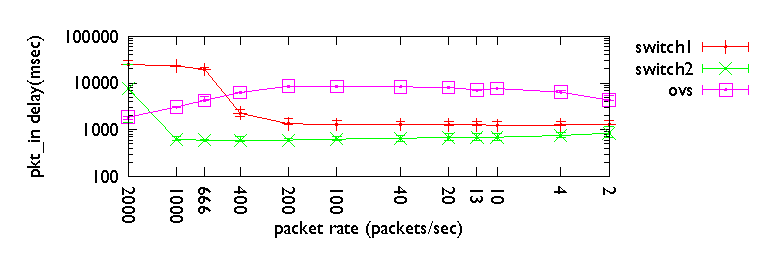
\includegraphics[width=0.99\textwidth]{pkt_in_delay}}
    \subfigure[Packet out message latenct]
	{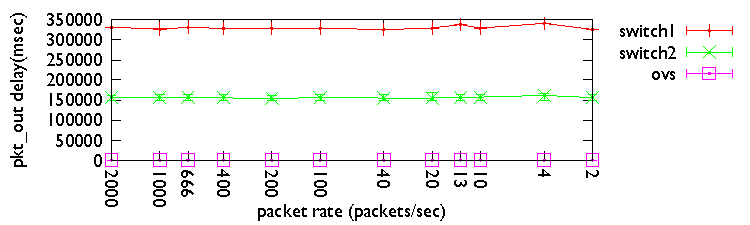
\includegraphics[width=0.99\textwidth]{pkt_out_delay}}
  \end{center}
  \caption{Latency to intercept or inject a packet using the \of protocol}
  \label{fig:pkt_in_out_delay}
\end{figure}

\of protocol permits a controller to intercept or inject traffic over the
control plane. This functionality allowed in the initial design of the \of
controller to be reactive and handle traffic on a per-flow basis. Packet
injection allows the controller to interact with connected network hosts. The
interception mechanism in \of has been reported in the initials deployments of
the protocol to cause significant slow-down in the control plane and led to
switch disconnection at high data rate~\cite{Kobayashi:vn}. This is a direct
consequence of the silicon design in current \of switches, that develop such
functionality as an low-frequency exception mechanism. In order to characterise
this functionality, we develop a simple experiment using \oflops that sends
packets at a specific rate and measure the latency of the switch to process
them. In Figure~\cite{fig:pkt_in_out_delay}, we show the latency induced on
packets both for Packet\_in and Packet\_out messages. We omit in this experiment
Switch 3 as this functionality maxed out its CPU utilisation and after a few seconds
made the switch unresponsive over the control channel. For packet\_out messages,
the switches rate limit through the tcp connection channel the rate of messages
received and as a result they provide a constant performance. For packet\_in
messages, we observe a diverse behaviour between hardware switches at high
packet rates. For Switch 1, packet loss and latency gets high for traffic rates 
above 400 packets per second. Additionally, we noticed that the switch is able to 
process a maximum of 500 packets/sec. For Switch 2 latency and packet loss are 
significantly lower and stable. Switch 2 faced problem to process packet  
important packet at high rates of 2000 packets per second. OpenVSwitch, has a high 
but stable latency for any tested data rates. 

\subsection{Flow table update rate}\label{sec:results-rate}

% So far, we get packet modification primitives and the expected performance that software/hardware can/should deliver.
% 
\begin{figure}[ht]
  \begin{center}
    \subfigure[OpenVSwitch (log-log scale)]
    {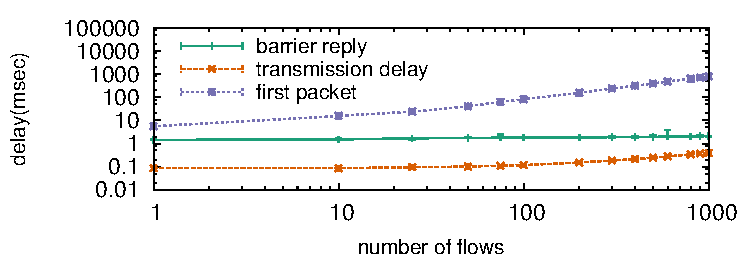
\includegraphics[width=0.99\textwidth]{openvswitch_mod_flow_exact_comparison}}
    \subfigure[Switch1 (log-log scale)]
	{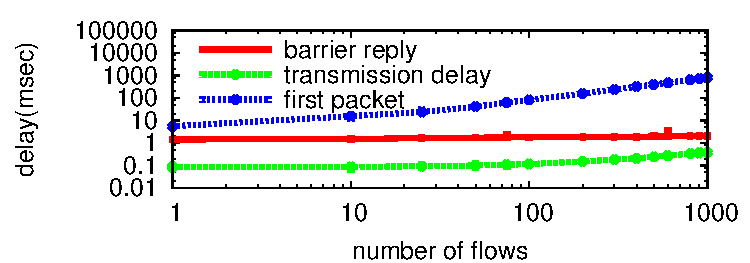
\includegraphics[width=0.99\textwidth]{nec_mod_flow_exact_comparison}}
  \end{center}
  \caption{Flow entry insertion delay: as reported using the
    \texttt{barrier} notification and as observed at the data
    plane.}
  \label{fig:flow_insertion_comparison}
\end{figure}

The flow table is a central component of an OpenFlow switch and is the
equivalent of a Forwarding Information Base (FIB) on routers. Given the
importance of FIB updates on commercial routers, e.g., to reduce the impact of
control plane dynamics on the data plane, the FIB update processing time of
commercial routers provide useful reference points and lower bounds for the time
to update a flow entry on an OpenFlow switch. The time to install a new entry on
commercial routers has been reported in the range of a few hundreds of
microseconds~\cite{shaikh-igp}.

OpenFlow provides a mechanism to define barriers between sets of
commands: the \texttt{barrier} command. According to the OpenFlow
specification~\cite{openflow-spec}, the barrier command is a way to be
notified that a set of OpenFlow operations has been completed. Further, 
the switch has to complete the set of operations issued prior to the barrier 
before executing any further operation. If the OpenFlow implementations 
comply with the specification, we expect to receive a barrier notification for 
a flow modification once the flow table of the switch has been updated, 
implying that the change can be seen from the data plane.

We check the behavior of the tested OpenFlow implementations,
finding variation among them. For OpenVSwitch and Switch1,
Figure~\ref{fig:flow_insertion_comparison} shows the time to install a
set of entries in the flow table. The NetFPGA-based switch results
(not reported) are similar to those of Switch1, while Switch2 and Switch3 
are not reported as this OpenFlow message is not supported by the firmware. 
For this experiment, \oflops relies on a stream of packets of 100 bytes at
a constant rate of 10Mbps that targets the newly installed flows in a
round-robin manner. The probe achieves sufficiently low inter-packet
periods in order to measure accurately the flow insertion time.
%With such a probe stream, we obtain an inter-packet
%period of less than 100$\mu$s, adequate for measuring any change in
%the flow-insertion time.

In Figure~\ref{fig:flow_insertion_comparison}, we show three different
times. The first, {\it barrier notification}, is derived by measuring the time 
between when the \textbf{first insertion command} is sent by the \oflops 
controller and the time the barrier notification is received by the PC. The 
second, {\it transmission delay}, is the time between the first and 
last flow insertion commands are sent out from the PC running \oflops. 
The third, {\it first packet}, is the time between the \textbf{first insertion
 command} is issued and a packet has been observed for the last of
the (newly) inserted rules. For each configuration, we run the
experiment 100 times and Figure~\ref{fig:flow_insertion_comparison}
shows the median result as well as the $10^{th}$ and $90^{th}$ percentiles 
(variations are small and cannot be easily viewed).
%\todo{point that the error
%  bounds are tight and cannot easily viewed on the graph}

From Figure~\ref{fig:flow_insertion_comparison}, we observe that even
though the {\it transmission delay} for sending flow insertion commands 
increases with their number, this time is negligible when compared with 
data plane measurements ({\it first packet}). Notably, the {\it barrier notification} 
measurements are almost constant, increasing only as the transmission delay 
increases (difficult to discern on the log-log plot) and, critically, this operation 
returns before any {\it first packet} measurement. This implies that the way
the {\it barrier notification} is implemented does not reflect the time when 
the hardware flow-table has been updated.

In these results we demonstrate how \oflops can compute per-flow
overheads. We observe that the flow insertion time for Switch1
starts at $1.8$ms for a single entry, but converges toward an
approximate overhead of $1$ms per inserted entry as the number of
insertions grows.

%%%%%%%%%%%%%%%%%%%%%%%%%%%%%%%%%%%%%%%%%%%%%%
\subsubsection*{Flow insertion types}
%%%%%%%%%%%%%%%%%%%%%%%%%%%%%%%%%%%%%%%%%%%%%%

\begin{figure}[h]
  \begin{center}
    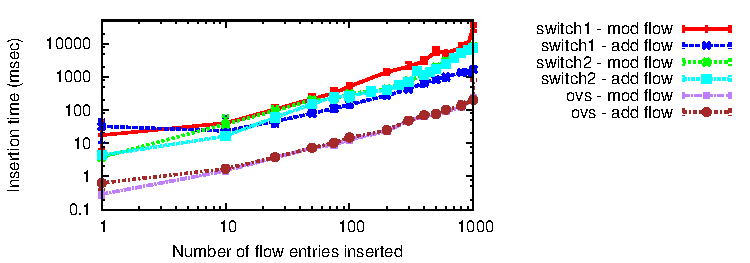
\includegraphics[width=0.80\textwidth]{flow_insertion_delay}
  \end{center}
  \caption{Delay of flow insertion and flow modification, as observed
    from the data plane (log-log scale).}
  \label{fig:flow_insertion_delay}
\end{figure}

We now distinguish between flow insertions and the modification of existing flows.  
With OpenFlow, a flow rule may perform exact packet matches or use wild-cards to 
match a range of values. Figure~\ref{fig:flow_insertion_delay} compares the flow
insertion delay as a function of the number of inserted entries. This is done for the 
insertion of new entries and for the modification of existing entries.

These results show that for software switches that keep all entries in memory, the 
type of entry or insertion does not make a difference in the flow insertion time.
Surprisingly, both Switch1 and Switch2 take more time to modify existing flow entries 
compared to adding new flow entries.  For Switch1, this occurs for more than 10 new 
entries, while for Switch2 this occurs after a few tens of new entries.
After discussing this issue with the vendor of Switch2, we came to the
following conclusion: as the number of TCAM entries increases, updates
become more complex as they typically requires re-ordering of existing
entries.

Clearly, the results depend both on the entry type and implementation.
For example, exact match entries may be handled through a hardware or
software hash table. Whereas, wild-carded entries, requiring support
for variable length lookup, must be handled by specialized memory
modules, such as TCAM. With such possible choices and range of
different experiments, the flow insertion times reported in
Figure~\ref{fig:flow_insertion_delay} are not generalizable, but
rather depend on the type of insertion entry and implementation.

% %%%%%%%%%%%%%%%%%%%%%%%%%%%
\subsection{Flow monitoring}\label{sec:results-monitoring}
% %%%%%%%%%%%%%%%%%%%%%%%%%%%

The use of OpenFlow as a monitoring platform has already been
suggested for the applications of traffic matrix
computation~\cite{opentm-pam,tm-presto} and identifying large traffic
aggregates~\cite{openflow-measurement-hotice}. To obtain direct
information about the state of the traffic received by an OpenFlow
switch, the OpenFlow protocol provides a mechanism to query traffic
statistics, either on a per-flow basis or across aggregates matching
multiple flows and supports packet and byte counters. 
%The result of a query returns packet and byte
%counters, either for the matched flows individually or for the
%aggregate.

We now test the performance implications of the traffic statistics reporting 
mechanism of OpenFlow. Using \oflops, we install flow entries that match 
packets sent on the data path. Simultaneously, we start sending flow statistics 
requests to the switch. Throughout the experiment we record: the delay getting 
a reply for each query, the amount of packets that the switch sends for each 
reply and the departure and arrival timestamps of the probe packets.

Figure~\ref{fig:stat_request} reports the time to receive a flow
statistics reply for each switch, as a function of the request
rate. Despite the rate of statistics requests being modest, quite high
CPU utilization results for even a few queries per second being
sent. Figure~\ref{fig:stat_request} reports the switch-CPU utilization
as a function of the flow statistics inter-request time. Statistics
are retrieved using SNMP. Switch3 is excluded for lack of SNMP
support.

\begin{figure}[h]
  \begin{center}
    \subfigure[Reply time.]
    {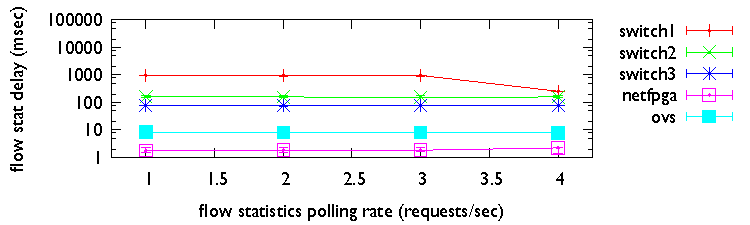
\includegraphics[width=0.99\textwidth]{flow_stats_delay}}
    \subfigure[CPU utilization.]
      {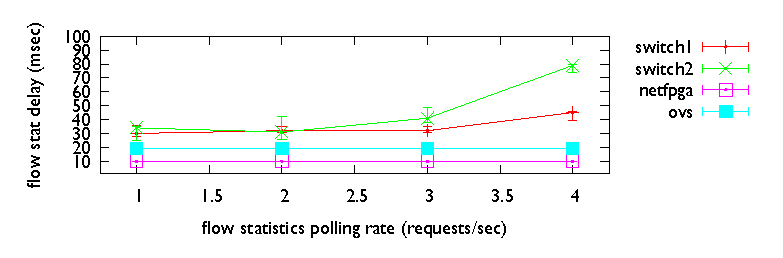
\includegraphics[width=0.99\textwidth]{flow_stats_cpu}\label{fig:stat_request_cpu}}
  \end{center}
  \caption{Time to receive a flow statistic (median) and corresponding CPU utilization.}
  \label{fig:stat_request}
\end{figure}

From the flow statistics reply times, we observe that all switches have (near-)constant 
response delays: the delay itself relates to the type of switch.
As expected, software switches have faster response times than
hardware switches, reflecting the availability of the information in memory
without the need to poll multiple hardware counters. These consistent response
times also hide the behavior of the exclusively hardware switches
whose CPU time increases proportionally with the rate of requests.  We
observe two types of behavior from the hardware switches: the switch
has a high CPU utilization, answering flow-stats requests as fast as
possible (Switch2), or the switch delays responses, avoiding
over-loading its CPU (Switch1). Furthermore, for Switch1,
we notice that the switch is applying a pacing mechanism on its
replies. Specifically, at low polling rates the switch splits its
answer across multiple TCP segments: each segment containing statistics for a
single flow.  As the probing rate increases, the switch
will aggregate multiple flows into a single segment. This suggests that 
independent queuing mechanisms are used for handling flow statistics 
requests. Finally, neither software nor NetFPGA switches see an 
impact of the flow-stats rate on their CPU, thanks to their significantly 
more powerful PC CPUs (Table~\ref{tbl:switch_list}).

%%%%%%%%%%%%%%%%%%%%%%%%%%%%%%%%%%%%%%%%%
\subsection{OpenFlow command interaction}\label{sec:results-interactions}
%%%%%%%%%%%%%%%%%%%%%%%%%%%%%%%%%%%%%%%%%

% why is it important this experiment

An advanced feature of the OpenFlow protocol is its ability to
provide applications with, e.g., flow arrival notifications from the 
network, while simultaneously providing fine-grain control of 
the forwarding process. This permits applications to adapt
in real time to the requirements and load of the
network~\cite{plug_n_serv,Yap09}. Under certain OpenFlow usage
scenarios, e.g., the simultaneous querying of traffic statistics and
modification of the flow table, understanding the behavior of the data
and control plane of OpenFlow switches is difficult without advanced
measurement instrumentation such as the one provided by \oflops. 
%One 
%of the strengths of \oflops is that is enables the development of custom scenarios
%that stress specific aspects of the OpenFlow control or data path.

Through this scenario, we extend Section~\ref{sec:results-rate} to show 
how the mechanisms of traffic statistics extraction and table manipulation 
may interact. Specifically, we initialize the flow table with 1024 exact
match flows and measure the delay to update a subset of 100 flows. 
Simultaneously, the measurement module polls the switch for full table 
statistics at a constant rate. The experiment uses a constant rate 10Mbps 
packet probe to monitor the data path, and polls every 10 seconds for SNMP 
CPU values.

\begin{figure}[t!!]
  \begin{center}
    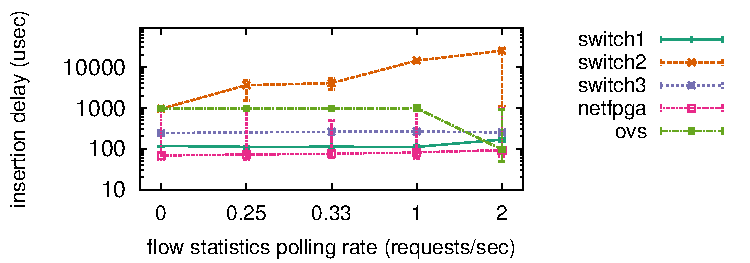
\includegraphics[width=0.99\textwidth]{interaction_test}
  \end{center}
  \caption{Delay when updating  flow table while the controller polls
    for statistics.}
  \label{fig:interaction_test}
\end{figure}

In this experiment, we control the probing rate for the flow statistics 
extraction mechanism, and we plot the time necessary for the modified 
flows to become active in the flow table. For each probing rate, we
repeat the experiment 50 times, plotting the median, $10^{th}$ and 
$90^{th}$ percentile. In Figure~\ref{fig:interaction_test} we can see
that, for lower polling rates, implementations have a near-constant
insertion delay comparable to the results of Section~\ref{sec:results-rate}.
For higher probing rates on the other hand, Switch1 and Switch3 do 
not differ much in their behavior. In contrast, Switch2 exhibits a noteworthy 
increase in the insertion delay explained by the CPU utilization increase
incurred by the flow statistics polling (Figure~\ref{fig:stat_request_cpu}). Finally,
OpenVSwitch exhibits a marginal decrease in the median insertion delay
and at the same time an increase in its variance. We believe this behavior 
is caused by interactions with the OS scheduling mechanism: the constant 
polling causes frequent interrupts for the user-space daemon of the switch, 
which leads to a batched handling of requests.

% \subsection{Timer precision} As part of each flow modification the
% protocol defines that the controller is able to define an expiration
% value for the flow. When a flow is expired, it is removed from the
% table. The protocol supports two different mechanism to define the
% timeout of a flow. Timeouts can be defined either based on the
% insertion time or the last time that the flow was used. The
% definition of the precision of this mechanism would be beneficial to
% applications that require high precision from the routing mechanism.
% In order to address the precision of the mechanism we are developing
% an experiment over the \oflops platform. The experiment utilizes 2
% ports of the switch and a single measurement probe with constant all
% field and random destination IP. During initialization the switch is
% initialized with a single wildcard flow that output packets to port
% 2. At time t=10 sec since the start of the experiment the controller
% sends an ensemble of exact match rules with different destination
% IP's and a hard expiration delay of 10 seconds. All the flows of the
% ensemble contain a single action which outputs packets on port
% 1. The experiments terminate when we receive all the flow expiration
% messages from the switch. During the experiment we log for each flow
% the time at which we received the first and last packet of the
% measurement probe for each destination IP. In the experiment we
% export as a parameter the number of flows send to the switch. For
% each number of flows we rerun the experiment for 20 times. In Figure
% \ref{fig:timer_precision} we present the results of our
% experiment. For each number of flows we plot an errorbar with the
% minimum, maximum and medium of the maximum error in the timeout of a
% flow based on the results of the packet timestamps of the
% measurement probe.
% \subsubsection*{Results}
% \subsection{Simulating a reactive switch} Simulate a Nox like
% behaviour and measure the time send at each stage of the flow
% insertion process. export as parameters the rate we send packets and
% the number of flows inserted.
% \subsubsection*{Results}
% LocalWords:  OpenFlow Oflops IP VLAN balancers SDNs virtualization NetFPGA th
% LocalWords:  UDP Mbps Gbps multiport timestamp OpenVSwitch dev dest src addr

% LocalWords:  NIC ToS TCP pcp interpacket TCAM lookup SNMP CPUs parameterising


\section{\sdnsim introduction} \label{sec:sdnsim-intro}

In the SDN paradigm, backward-compatible evolvability of computer networks is
achieved through the distribution of control to external programmable units. The
protocols provides all required mechanisms in order to allow a remote entity to
get sufficient forward plane feedback and control the forwarding process at a very fine
level. So far the trend in \of design is to aggregate control in a single
control unit, in order to have a single point of control in the network. This
aggregation permits on one hand to achieve higher optimality in forwarding
policy, while on the other hand the logic can be developed in richer
programming environments, than the embedded systems usually found in current
network devices.

The ability to distribute control over multiple functional units, in conjunction
with the complex nature of network stacks, as well as the diverse behaviour of
\of switch and controlling platforms, reduces the ability of developers to
predict the behaviour of an SDN design. In order to reason on correctness,
developers must build realistic small scale experiments, and larger scale 
experiments in order to reason on performance. In the related literature on network
evaluation there have been two main experimental approaches:
\emph{realistic testbed} and \emph{simulation}.

In the realistic experimentation approach, scientists try to reconstruct the
exact properties of the deployment environment. This approach provides an
optimal measurement environment the provides full control of the parameter of
the experiment, but has a significant overhead in resources and configuration
time. Experimenting with a real datacenter would require a high number of
machines that implement full functionality of the target environment, large
interconnection planning and careful metrication and analysis of the resulting
system. These requirements scale badly as the number of network hosts increases.
In order to reduce resource costs, the research community has developed shared
testbeds~\todo{add some pointers.}.  Such testbeds though limit the capability
of users to control measurement noise and network topologies. 

In the simulation approach, researchers replace some part of the functionality
of the system by a simpler model. The goals of such an approach is to reduce the
complexity of the experiment, and achieve scalability for large network sizes. This
approach has two main drawbacks. Firstly, the fidelity of the results depends
extensively on the reality of the assumptions of the model. Secondly, in order to
simulate appropriately the network, the users usually need to rewrite the logic
of their experiments in order to fit the abstraction of the underlying models.
For example, in order to simulate \of-based network currently there is no
off-the-self simulation platform to support the protocol. An \of architect is
required to reimplement its \of logic in order to experiment with architectural
designs. 

\sdnsim~\footnote{\oflops is under GPL licence and can be downloaded from
  \url{http://github.com/crotsos/sdnsim/}} is a novel framework, that bridges
the two domains of experimentation and provides an \of specific development
environment. The framework is written in OcaML, a high performance functional
language, and extends the functionality of the
Mirage~\footnote{\mirageurl} library OS. Developers can
  implement the required functionality of their network design and at the
  compilation step select the target experiment type. \sdnsim provides two
  target options: a simulation target, that runs the Mirage code
  on top of the ns-3 simulation environment, and a realistic target, that build
  and deploys each node of the simulation as a DomU VM and configuration
  resource allocation using xen's API. 

% SDNsim is an ensemble of libraries that provide a simple simulation abstraction
% layer to define and implement SDN deployment scenarios. The platform aims to
% translate network definitions into concrete experiment implementations. More
% specifically, the translation process can generate high-accuracy
% event-driven simulations over the NS3 platform as well as real-time emulation
% by interconnecting DomU virtual machines over the Xen platform.  Here, we
% define the architecture of the platform, describe the library
% applications that the platform supports, provide an initial performance
% evaluation, and conclude with the required functionality. 
% 
% The source code can be found at \url{http://github.com/crotsos/mirage}; it
% has been successfully tested under both Linux and Mac OSX. 
% Details on the required step to install and try the code are forthcoming.
% For Linux, the process is fairly straightforward; 
% for MacOS X, a patch for the NS3 code is required to compile all the required modules. 

\section{Mirage Library OS} \label{sec:mirage-intro}

\begin{figure}
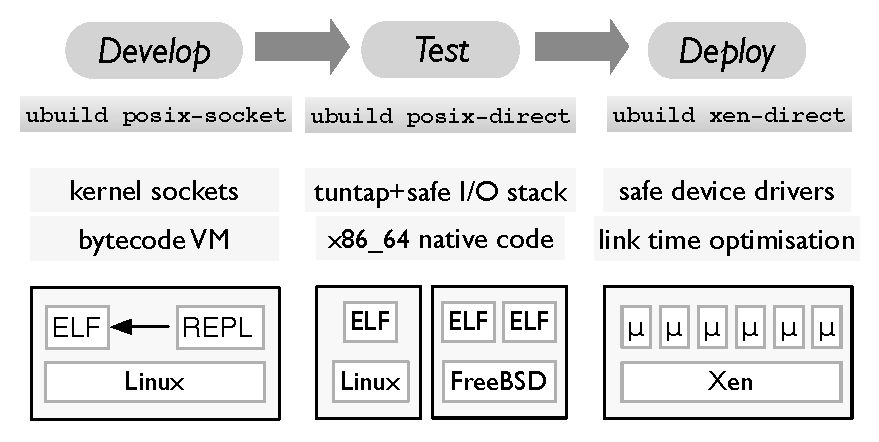
\includegraphics[width=0.9\textwidth]{mirage-toolchain}
\caption{Specialising a \mirage application through recompilation alone, from
  interactive UNIX Read-Eval-Print Loop, to reduce dependency on the host
  kernel, and finally a unikernel VM.}
\label{fig:mirage-toolchain}
\end{figure}

Cloud computing has revolutionized the way the business use IT infrastructures
as well as the way we develop distributed computing applications. The
abstraction is straightforward. A third party entity takes responsibility to
maintain a datacenter. This infrastructure, is partitioned into smaller virtual
computational units which clients can rent in order to run their applications.
The elegance of this model is based on simplicity of the abstraction that the
cloud provider provides to the user and the ability to port existing services
running on a personal computer or a server to the cloud platform. 

Although the simplicity of the exposed abstraction, the cloud architecture
consist of a complex set of processing layers. A single application VM would
include: i) the virtualization runtime layer, ii) the guest OS kernel layer,
iii) A language runtime layer (POSIX, JVM etc.) iv) user-space
thread layer. This layer complexity, although it provides excellent backwards
compatibility for existing datacenter applications, it makes the process of
optimisation, debugging as well as security difficult, while there is a
significant overlap on the functionality provided by each layer. 

Mirage is a clean-slate application synthesis framework that allows users to
compile application to a single bootable VM image. Mirage relies on the idea of
library OS; functionality is separated into logical modules which integrates in
a resulting binary, only if needed by the code. As a result, Mirage is able to
generate small size VM images which additionally are fast to boot. Although, 
OCaml is a functional language, it is able to generate highly performand binary
code and application specific microbenchmarks has shown performance to be
compare to c code implementations. In order to
minimize processing layers, IO operations are coded on top of the NetFront
device abstraction provided by Xen, while the OS is using extensively zero-copy
mechanisms and exposes directly the pages of the shared memory ring to
application space, over a simple abstraction that enforces memory boundaries.

Mirage executes OCaml code over a specialised language runtime modified in two
key areas: memory management and concurrency. Because of the single process
nature of Mirage images, the OS uses a single address space, separated between
the text and data section of the program and the runtime heap. Because the
program code is immutable during runtime, Mirage can lock write access to
executable memory space, thus mitigating buffer overflow attacks. Additionally,
this mechanism removes the requirement of Address Space Randomization (ASR),
which simplifies and makes more efficient memory management.  To provide
concurrency beyond Xen IO polling function, Mirage integrates the Lwt
cooperative threading library~\cite{lwt}. This internally evaluates blocking
functions into event descriptors to provide straight-line control flow for the
developer.  Written in pure OCaml, Lwt threads are heap-allocated values, with
only the thread main loop requiring a C binding to poll for external events.
Mirage provides an evaluator that uses Xen polling to listen for events and wake
up lightweight threads. The VM is thus either executing OCaml code or blocked,
with no internal preemption or asynchronous interrupts. The main thread
repeatedly executes until it completes or throws an exception, and the domain
subsequently shuts down with the VM exit code matching the thread return value.
A useful consequence is that most scheduling and thread logic is contained in an
application library, and can thus be modified by the developer as they see fit. 

In order to provide basic system programming capabilities, Mirage OS provides
two core modules, named Net and OS, that implement and expose the required
functionality for networking and device management, respectively. The API is
similar to the API provided by the Unix model from OCaml; developers can modify
their code and compile existing applications to Mirage VMs. Due to the
simplicity of the OS and Net modules, Mirage provides the ability to compile
code to other target backends, apart from the Xen platform. Specifically, Mirage 
can generate UNIX binaries, using both the POSIX library network functionality 
and raw sockets, and even Javascript executables that run in a browser. There is
also currently an effort to port Mirage in the FreeBSD kernel as well as the
BareboneOS, an assembly written minimum OS. The diverse set
of deployment backends, provides to developers an environment to
test and optimize code gradually. Developers build initially their core logic over
the POSIX backend in order to test the correctness of the code, then they can
try their code over the Mirage default network stack, to perform a small scale
performance evaliation, and finally they can synthesize the resulting deployable 
Xen Image~\ref{fig:mirage-toolchain}.

\section{\sdnsim design} \label{sec:sdnsim-design}

\lstset{language=XML,
numberstyle=\footnotesize,
basicstyle=\ttfamily\footnotesize,
captionpos=b,
}
\begin{lstlisting}[caption={A sample \sdnsim configuration file interconnecting
  a server and a client host},label={lst:sdnsim-conf}]
<?xml version="1.0" encoding="ISO-8859-1"?>
<topology module="Simple_tcp_test" backend="ns3-direct" 
    duration="30">
  <modules>
    <library>lwt</library>
    <library>lwt.syntax</library>
    <library>cstruct</library>
    <library>cstruct.syntax</library>
    <library>mirage</library>
    <library>mirage-net</library>
    <library>pttcp</library>
  </modules>
  <node name="host1" main="host_inner"> 
    <param>1</param>
  </node>
  <node name="host2" main="host_inner"> 
    <param>2</param>
  </node>
  <link src="host1" dst="host2" delay="10" rate="100" 
    queue_size="100" pcap="false"/>
</topology>
\end{lstlisting}

\begin{figure}
\centering
\subfigure[NS3]{
 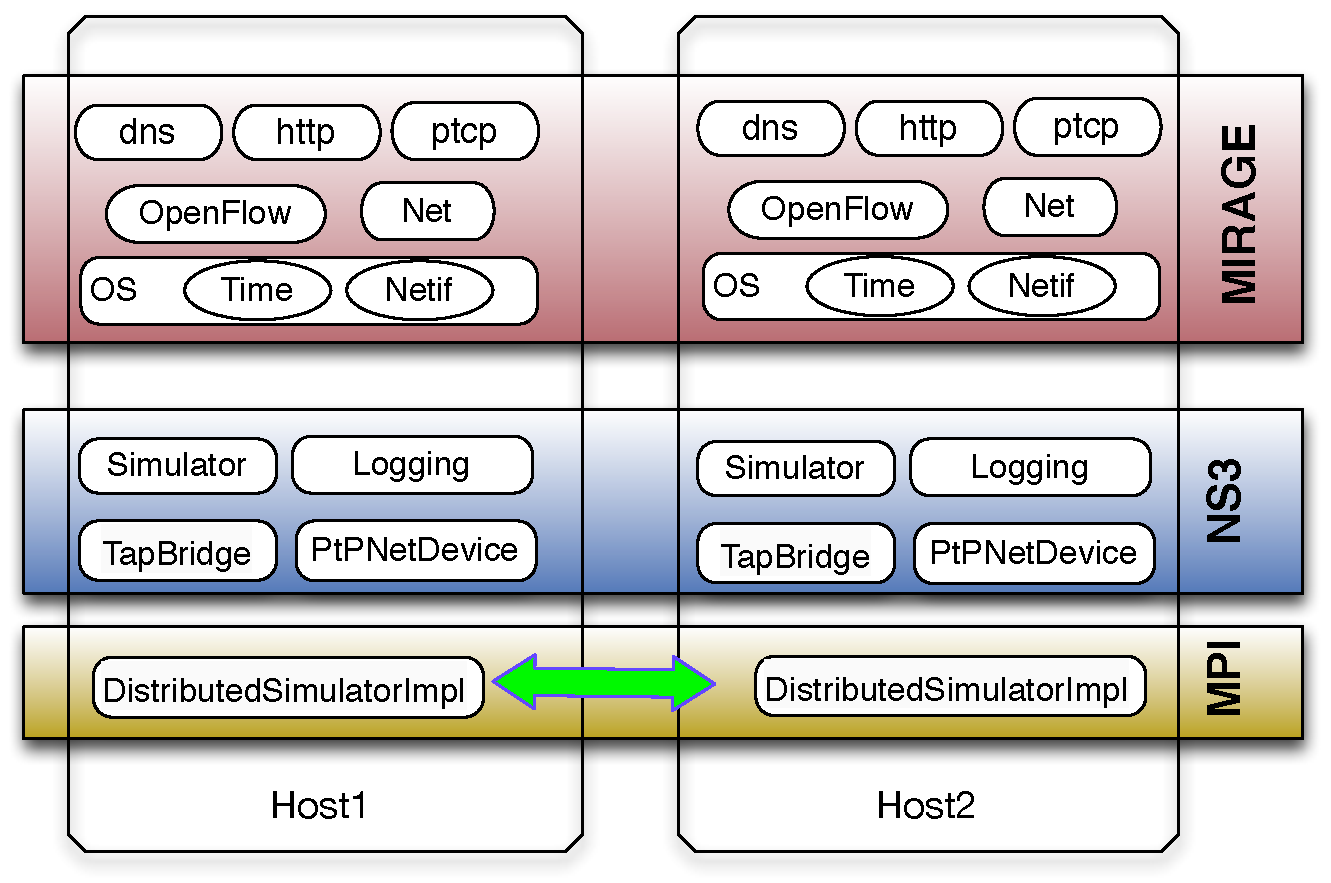
\includegraphics[width=0.45\textwidth]{sdnsim-arch-ns3}
 \label{fig:sdnsim-arch-ns3}}
\subfigure[Xen] {
 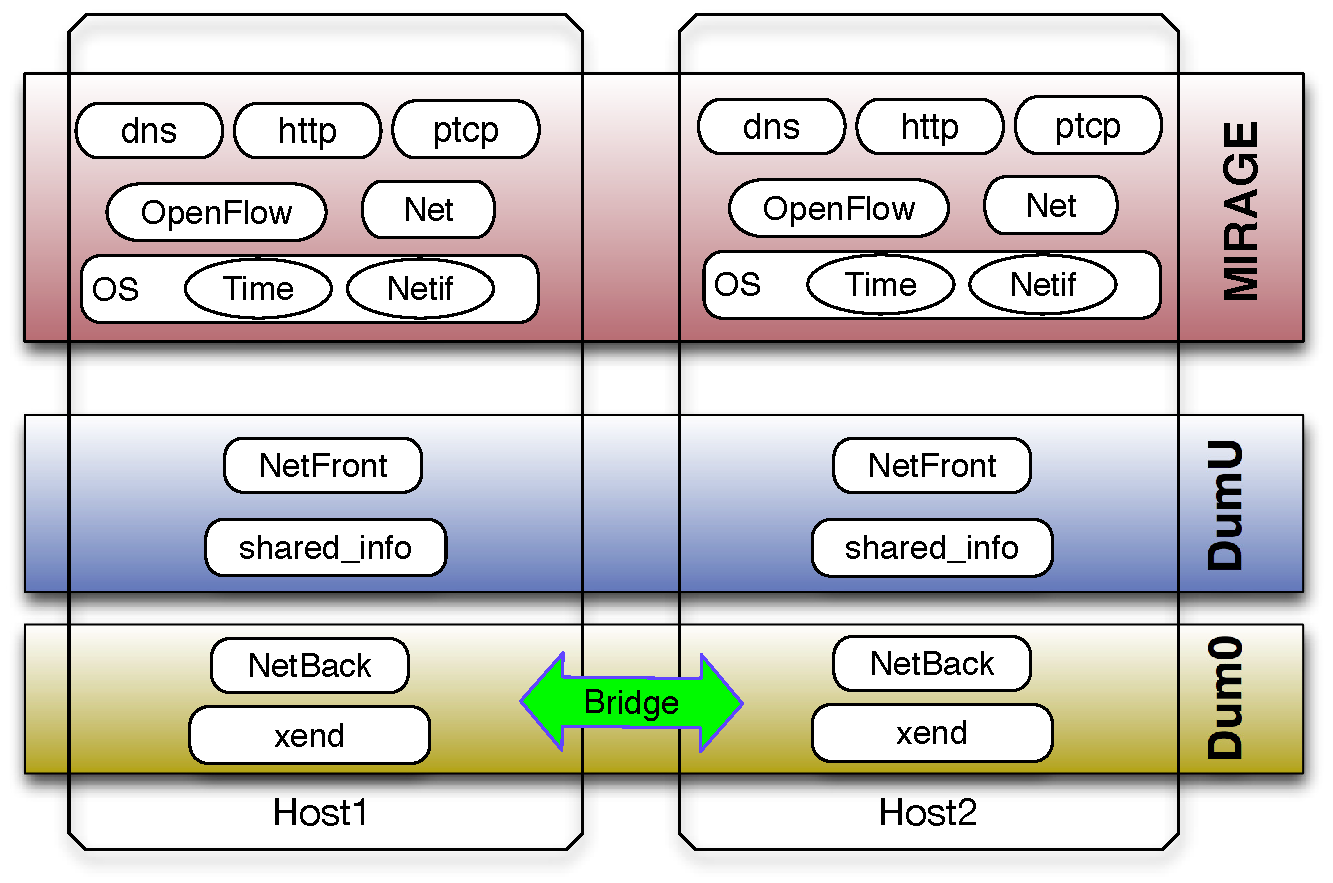
\includegraphics[width=0.45\textwidth]{sdnsim-arch-xen}
 \label{fig:sdnsim-arch-xen}}
\caption{\sdnsim host internal architecture: NS3
  simulation~\ref{fig:sdnsim-arch-ns3} and xen real-time
  emulation~\ref{fig:sdnsim-arch-xen}.}
\label{fig:sdnsim-arch}
\end{figure}

For the user perspective, the core of \sdnsim consists on a single executable
that works as one more OCaml build system. Developers write their OCaml code in
order to define the functionality of network nodes, and use a single xml file in
order to describe the network topology and match functionality to network hosts.
A sample xml file is presented in Listing~\ref{lst:sdnsim-conf}. The
configuration describes a simple client~(host1)~-~server~(host2) configuration.
For an experiment definition, developers needs to define, at minimum,  the core
code module~(topology@module), the target executable~(topology@backend) and the
duration of the experiment~(topology@duration). In order to define a host,
\sdnsim uses a host xml entity. For each host users must define the host
name~(node@name) and the host main function~(node@main), while a number of named
parameters~(node/param) can be passed to the main function. Finally, developers
can define links between hosts~(link@src, link@dst) along with the
device~(link@queue\_size, link@pcap) and propagation properties~(link@rate,
link@delay), using the link xml entity. Links can be used also to integrate
external network interfaces in the simulation, in order to allow the experiment to
interact with entities outside of the experiment scope.

The functionality of a node in the \sdnsim platform can be split in 3 layers.  A
simple representation of the architecture of an \sdnsim host can be seen in
Figure~\ref{fig:sdnsim-arch}.  At the top layer of the host is the application
logic of the host. This layer is defined by the developer, and define the
traffic load of the network and its forwarding logic. In order to allow
realistic traffic patterns, \sdnsim can reuse all the application protocol libraries
supported in the \mirage platform, namely dns, http, ssh and \of. Additionally,
we have re-implemented in OCaml the pttcp tcp test tool functionality~\ref{pttcp},
in order to allow model driven TCP flow generation. 

In the middle layer of the host architecture, we reuse the network library and
the OS abstraction defined by the Mirage platform. These libraries are mapped in
the lower layer of the respective backend. Because this platforms aims to
develop an \of capable simulation platform, the main focus for the integration
between the two lower layer is the fidelity in network functionality and time
consistency. Currently, \sdnsim supports two backends, {\it NS3} and {\it Xen}.
In order to implement the lower layer interaction, a different strategy has been 
followed for each backend. 

\subsection{Xen}

In order to run a Mirage Xen Image, the project provides a simple PV Boot
mechanism. The mechanism initializes a VM with a single virtual CPU, loads the
Xen event channel and jumps to a main function of the VM. The main function
firstly enumerates IO devices and notifies the application and then proceeds to the
main threading scheduling logic. As we have mentioned earlier, the threading
mechanism in Mirage is based on Lwt, a language extension which enables seamless
event-driven asynchronous programming. Using Lwt suntax, each closure can be
noted as blocking, and spawn a new lwt thread. At the lowest level, an lwt
thread is either tied to a blocking IO request, or a time dependent event. Using
this information, the scheduling logic works as follow: If no sleeping thread
is currently available to resume, the schduler calculated the
time left until the next time event and uses it as the timeout parameter for the
IO blocking method (named {\emph domainpoll}) provided by the Xen platform.
Domainpoll registers interest to the respective event handler and ask the Xen
scheduler to put the VM to sleep until either an event occurs or the timeout
option expires.

In order to integrate the clock of a mirage instance with the global clock of
the Xen platform, each time request is mapped to the time counter provided by Xen
shared\_info struct. In respect to the network functionality of Mirage, network
packets are mapped as IO events on the network device of the NetFront driver.
Using this simple logic, users can develop highly functional appliances which
can be deployed as small factor image over the Xen platform.

Further, in order to express network topologies over the Xen platform, 
\sdnsim takes advantage of the Xen API provided by the
latest version of the Xen platform. The API provides the ability to fully
control functionality and resource allocation for each VM running on a Xen
domain. \sdnsim, using the Xen API, is able to implement network 
topologies through vif bridging between hosts, while link
rate and propagation delay can be encoded in the vif definition. 
When \sdnsim  is instructed to run a real-time experiment, it firstly compiles 
all required VM images, creates the appropriate host definition and network
topologies and when the configuration step is completed it can fire the
experiment.

\subsection{NS3}

NS3 is a framework for discrete time packet driven network simulation. It
builds around a basic event-driven simulation engine and provides a set of
libraries that implement an extensive set of network applications, routing
protocols, data-link layer protocols and link emulations models. NS3 is widely
used in academia and is considered as the default simulation tool in the
domain of MANETs and wireless communications. 

Since the way that the NS3 platform is event driven and the scheduling mechanism
is hidden in the Simulation engine, we followed a different approach in order to
map \mirage functionality.
Firstly, in order to bridge the simulation clock with the Mirage host time, we have
mapped the gettimeofday functionality of the OS with the global Simulator
clock of the NS3 platform. Further, in order to provide accurate time events in
the \mirage platform we modified the main mechanism for time events in the
platform, the sleep function. Each sleep call is blocked and scheduled
as an NS3 timed event. The thread is resumed only when the simulator fires the
respective timed event. Finally, in order to make sure that any sleeping thread
is not paused for a long period, the OS schedules {\emph idle} timed events that
check for resume any yielded threads.

% link. We use this connection abstraction because the link state can 
% separated between hosts in order to enable distributed simulations. 

The networking functionality uses the simple link abstraction of a {\emph
  PointToPoint channel}. This model simulates a ppp link over a lossless medium,
a valid model for the full duplex non-shared medium of current network
datacenters. Traffic transmission, uses a single packet queue per network device
shared between the \mirage layer and the NS3 simulator engine.  The only
modification we make on the design of the ns3 link is to modify the network
queue functionality of the network device abstraction. The queue implement a
simple bidirectional feedback mechanism in order to avoid any buffer overflows,
as well as avoid queue polling to check if the queue has space for new packets.
For packet receipt, the NS3 device allows registering receipt callback to each
virtual network device. The packet demuxing callback implements logic to forward
packets to the appropriate listening thread.

% An important assumption of the current architecture that provides accuracy in
% simulation time is the blocking nature of the event-handling process. 
% In this way,
% the virtual clock will not increment while a host is processing an event and
% all processing complexity of hosts is assumed to incur negligible delays. 

A performance limitation that we faced during the development of the NS3 backend
for \sdnsim is the natural inability of the OCaml runtime to support
multi-threaded programming. This simplification provides more predictable
performance for the program, as the garbage collector doesn't have to manage
threads synchronisation, while scalability can be achieved through multiprocess
programs that synchronise through other IPC mechanisms. In order to make \sdnsim
scalable for large network sizes we followed a similar approach. For the
simulation engine we use DistributedSimulationImpl class, which uses message
passing techniques in order to coordinate multiple simulation
instances~\cite{Pelkey:2011ua}. This simulation mechanism uses a simple and
conservative clock synchronisation mechanism, that ensures that all events are
executed in order. 


\section{\sdnsim evaluation} \label{sec:sdnsim-precision}

In order to evaluate the performance of the \sdnsim platform we develop a number
of small scale microbenchmarks in order to evaluate the performance of the \of
protocol functionality as well as the performance of the NS-3 binding.
In~\cite{unikernel}, there is an exhaustive analysis of the performance of the
\mirage platform, which we omit from this section. In Section~\ref{sec:of-perf},
we use two off-the-self \of benchamarking platforms in order to characterise the 
performance of the controller and switch implementation. Further, in
Section~\ref{sec:sdnsim-ns3-perf} we characterise the scalability of the NS3 
backend.

% \subsection{\of library performance} \label{sec:of-perf}

\subsection{\mirage Controller}

We benchmark our controller library's performance through a simple
baseline comparison against two existing OpenFlow controllers, NOX and
Maestro. NOX~\cite{nox} is one of the first and most mature publicly available
\of controllers; in its original form it provides programmability through
a set of Python modules. In our evaluation we compare against both the master
branch and the \emph{destiny-fast} branch, a highly optimised version that
sacrifices Python integration for better performance. Maestro~\cite{maestro}
is an optimised Java-based controller that aims to achieve fairness among
switches. We compare these against the Mirage controller targeting two
different network backends: \emph{mirage-unix} targets the UNIX Sockets
backend and so uses the existing Linux TCP/IP stack, while \emph{mirage-xen}
targets the Xen hypervisor and runs as a domU virtual machine using the Mirage
TCP/IP stack.

Our benchmark setup uses the \emph{cbench}
application\footnote{\url{http://www.openflow.org/wk/index.php/Oflops}}. Each
emulated switch simultaneously generates \emph{packet-in} messages and the
program measures the throughput of the controller in processing these
requests. It provides two modes of operation, both measured in terms of
\emph{packet-in} requests processed per second: \emph{latency}, where only a single
\emph{packet-in} message is allowed in flight from each switch; and
\emph{throughput}, where each switch maintains a full 64\,kB buffer of
outgoing packet-in messages. The first measures the throughput of the
controller when serving connected switches fairly, while the second measures
absolute throughput when servicing requests.
                                                                       
We emulate 16 switches concurrently connected to the controller, each serving
100 distinct MAC addresses. We run our experiments on a 16-core AMD server
running Debian Wheezy with 40\,GB of RAM and each controller configured to use
a single thread of execution. We restrict our analysis to the single-threaded
case as Mirage does not yet support multi-threading. For each controller we
run the experiment for 120\,seconds and measure the per-second rate of
successful interactions. Table~\ref{tbl:controller} reports the average and
standard deviation of requests serviced per second.

Unsurprisingly, due to mature, highly optimised code, \emph{NOX fast} shows
the highest performance for both experiments. However, we note that the
controller exhibits extreme short-term unfairness in the throughput test.
\emph{NOX} provides greater fairness in the throughput test, at the cost of
significantly reduced performance. Maestro performs as well as NOX for
throughput but significantly worse for latency, probably due to the overheads
of the Java VM. Finally, Mirage throughput is somewhat reduced from NOX fast
but substantially better than both NOX and Maestro with both backends; the Xen
backend wins out over the UNIX backend due to reduction of layers in the
network stack. In addition, Mirage Xen achieves the best product of
performance and fairness among all tested controllers in the throughput test.
Comparing latency, both Mirage backends perform much better than Maestro but
suffer somewhat in comparison to NOX: we believe this is due to the lack of
optimisation in the Mirage TCP/IP stack.

\begin{table}\small
\newcommand\T{\rule{0pt}{2.6ex}}
\newcommand\B{\rule[-1.2ex]{0pt}{0pt}}
\centering
\begin{tabular} { l | r@{.}l r@{.}l | r@{.}l r@{.}l }
\hline
\T \multirow{2}{*}{Controller} 
   & \multicolumn{4}{c|}{Throughput (kreq/sec)}  
   & \multicolumn{4}{c}{Latency (kreq/sec)} \\
\B & \multicolumn{2}{c}{avg} & \multicolumn{2}{c|}{std. dev.} 
   & \multicolumn{2}{c}{avg} & \multicolumn{2}{c}{std. dev.} \\
\hline
\T NOX fast   & 122&6 & \quad{} 44&8 & 27&4 & \quad{} 1&4 \\
NOX           &  13&6 &  1&2 & 26&9 & 5&6 \\
Maestro       &  13&9 &  2&8 &  9&8 & 2&4 \\
Mirage UNIX   &  68&1 & 11&7 & 21&1 & 0&2 \\
\B Mirage Xen &  86&5 &  4&4 & 20&5 & 0&0 \\
\hline
\end{tabular}
\caption{\label{tbl:controller}OpenFlow controller performance.}
\end{table}

\subsection{\mirage Switch}

We also use the Oflops benchmark platform~\cite{oflops} to evaluate
performance of the Mirage switch implementation. We compare against the Open
vSwitch\footnote{\url{http://openvswitch.org}}~(OVS) kernel implementation, an
OpenFlow-enabled software switch implemented as a Linux kernel module. OVS is
currently used by many datacenter service providers to enable virtual machines
to be bridged in dom0, while its OpenFlow functionality is used by vendors to
implement OpenFlow firmware.

For this experiment we use two virtual machines, one running the Oflops code,
the other running the OpenFlow switch configured with three interfaces bridged
separately in dom0. One interface provides a control channel for the switch,
while the other two are used as the switch's data channels. This represents a
setup that might be used to enable an application to modify switch
functionality without affecting the network functionality in dom0. Using
Oflops, we generate packets on one of the data channels and receive traffic on
the other, having inserted appropriate flow table entries at the beginning of
the test. We run the test for 30\,seconds using small packets (100\,bytes) and
varying the data rate.

\begin{figure}
\centering
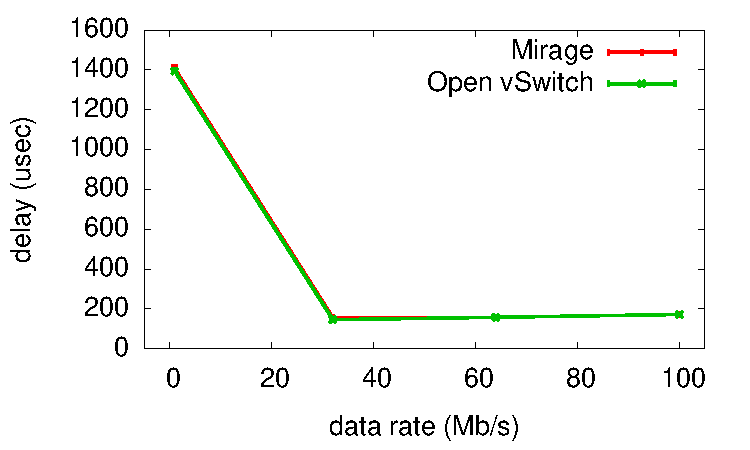
\includegraphics[width=\columnwidth]{switch-media-delay}
\caption{\label{fig:switch}Min/max/median delay switching 100\,byte packets
        when running the Mirage switch and Open vSwitch kernel module as domU
        virtual machines.}
\vspace{-2ex}
\end{figure}

Figure~\ref{fig:switch} plots as error boxes the min, median and max of the
median processing latency of ten test runs of the experiment. We can see that
the Mirage switch's forwarding performance is very close to that of Open
vSwitch, even mirroring the high per-packet processing latency with a probe
rate of 1\,Mb/s; we believe this is due to a performance artefact of the
underlying dom0 network stack. We omit packet loss due to space constraints,
but can report that both implementations suffer similar levels of packet loss.
However, the Mirage switch has a memory footprint of just 32\,MB compared with
the Open vSwitch virtual machine requirement of at least 128\,MB. We are
currently working toward better integration of the Mirage switch functionality
with the Xen network stack to achieve lower switching latency.

\subsection{NS-3 performance} \label{sec:sdnsim-ns3-perf}

In order to test the scaling properties of the NS3 backend we perform a simple
topology experiment~(Figure~\ref{Haris-Fig2}) with variable number of hosts.
The hosts are generated in pairs and are programmed to generate steady-state
full-rate TCP traffic between them.  We use two variations of the topology: A
centralised example where all hosts are  connected to a single switch, and a
localised example, where hosts are distributed between two switches and traffic
is local to the switch.Each switch is connected to an \of controller that
implements a learning switch. The experiment executes 30 seconds of simulation
time.

In Table~\ref{Haris-Table1}, we present the real execution time and the slowdown
factor of each simulation.  The results show that the platform can scale close
to linear the hosts of the simulation create small autonomous partition. In the
centralised example, the \of switch is the bottleneck of the simulation, as it
has to process sequentially all network events. In the distributed example, the
network event processing is distributed between the two switches of the
topology, thus achieving better simulation parallelization.

\begin{figure}
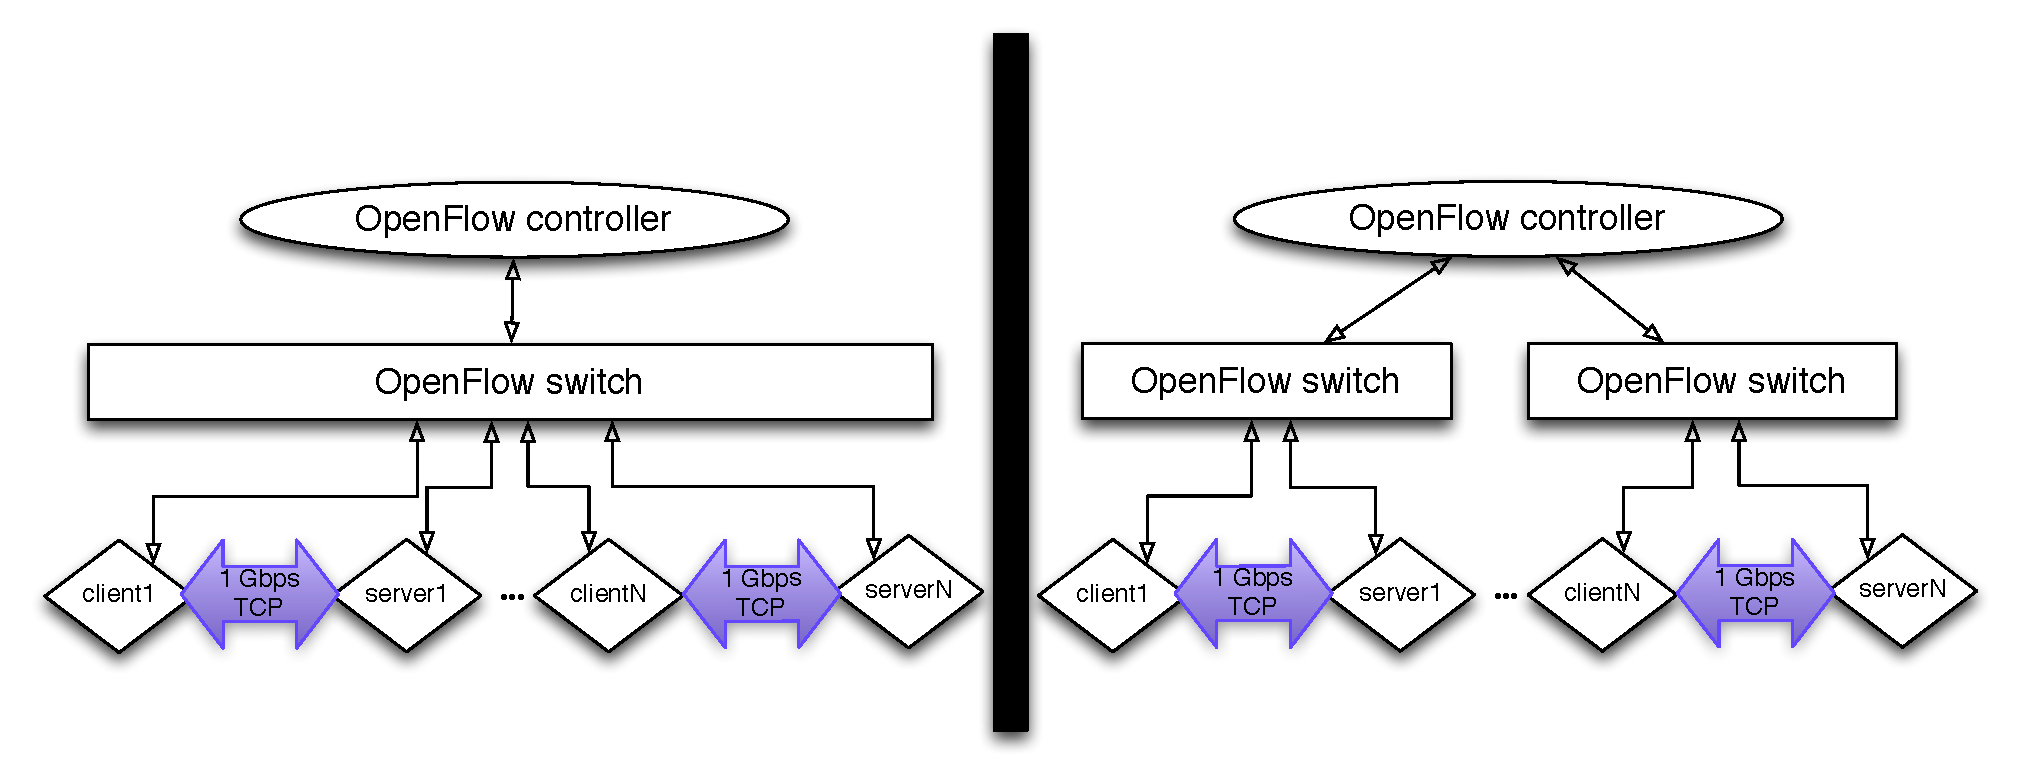
\includegraphics[width=0.9\textwidth]{sdnsim-topology}
\caption{Topology of two basic simulation scenarios for the SDNsim platform}
\label{Haris-Fig2}
\end{figure}

\begin{table}
\label{Haris-Table1}
\begin{center}
\begin{tabular}{|l|c|c|c|c|c|c|} \hline
&\multicolumn{3}{|c|}{Single Switch} & \multicolumn{3}{|c|}{two switches} \\
\cline{2-7}
Number of hosts & 2 & 8 & 12 & 4 & 8 & 12 \\
\hline 
Delay (in min) & 17 & 90 & 171 & 21 &50 & 82 \\
\hline
Slowdown factor & 34 & 180 & 242 & 42 & 100 & 164 \\
\hline 
\end{tabular}
\end{center}
\caption{\sdnsim simulation of a fat-tree topology over NS3 backend allows
  better scaling of the slowdown factor as the traffic is localised. }
\end{table}

\section{Security Tradeoffs on Datacenter Network Micro-control} \label{sec:rdsf-eval}

%%%%%%%%%%%%%%%%%%%%%%%%%%%%%%
\section{Summary and Conclusions}\label{sec:conclusion}
%%%%%%%%%%%%%%%%%%%%%%%%%%%%%%
  
We presented, \oflops, a tool that tests the capabilities and performance of 
OpenFlow-enabled software and hardware switches. \oflops combines advanced 
hardware instrumentation, for accuracy and performance, and provides an extensible 
software framework. We use \oflops to evaluate five different OpenFlow switch 
implementations, in terms of OpenFlow protocol support as well as performance.
%In our performance evaluation, we benchmark the packet processing, flow table
%modification and traffic statistics export functionalities of the switches.

We identify considerable variation among the tested OpenFlow implementations.
We take advantage of the ability of \oflops for data plane measurements to
quantify accurately how fast switches process and apply OpenFlow commands.
For example, we found that the barrier reply message is not correctly implemented,
making it difficult to predict when flow operations will be seen by the data plane.
Finally, we found that the monitoring capabilities of existing hardware switches 
have limitations in their ability to sustain high rates of requests. Further, at high 
rates, monitoring operations impact other OpenFlow commands.

We hope that the use of \oflops will trigger improvements in the
OpenFlow protocol as well as its implementations by various vendors.

%We also readily acknowledge this paper as a snapshot of work in
%progress; every set of results poses new questions but also the role
%of \oflops can evolve as new OpenFlow instantiations are introduced and
%existing ones refined; considerable opportunity exists for future
%work.

% LocalWords:  Oflops OpenFlow

%%% Local Variables: 
%%% mode: latex
%%% TeX-master: "../thesis"
%%% End: 
